% Options for packages loaded elsewhere
\PassOptionsToPackage{unicode}{hyperref}
\PassOptionsToPackage{hyphens}{url}
\PassOptionsToPackage{dvipsnames,svgnames,x11names}{xcolor}
%
\documentclass[
  letterpaper,
  DIV=11,
  numbers=noendperiod]{scrartcl}

\usepackage{amsmath,amssymb}
\usepackage{iftex}
\ifPDFTeX
  \usepackage[T1]{fontenc}
  \usepackage[utf8]{inputenc}
  \usepackage{textcomp} % provide euro and other symbols
\else % if luatex or xetex
  \usepackage{unicode-math}
  \defaultfontfeatures{Scale=MatchLowercase}
  \defaultfontfeatures[\rmfamily]{Ligatures=TeX,Scale=1}
\fi
\usepackage{lmodern}
\ifPDFTeX\else  
    % xetex/luatex font selection
\fi
% Use upquote if available, for straight quotes in verbatim environments
\IfFileExists{upquote.sty}{\usepackage{upquote}}{}
\IfFileExists{microtype.sty}{% use microtype if available
  \usepackage[]{microtype}
  \UseMicrotypeSet[protrusion]{basicmath} % disable protrusion for tt fonts
}{}
\makeatletter
\@ifundefined{KOMAClassName}{% if non-KOMA class
  \IfFileExists{parskip.sty}{%
    \usepackage{parskip}
  }{% else
    \setlength{\parindent}{0pt}
    \setlength{\parskip}{6pt plus 2pt minus 1pt}}
}{% if KOMA class
  \KOMAoptions{parskip=half}}
\makeatother
\usepackage{xcolor}
\setlength{\emergencystretch}{3em} % prevent overfull lines
\setcounter{secnumdepth}{-\maxdimen} % remove section numbering
% Make \paragraph and \subparagraph free-standing
\makeatletter
\ifx\paragraph\undefined\else
  \let\oldparagraph\paragraph
  \renewcommand{\paragraph}{
    \@ifstar
      \xxxParagraphStar
      \xxxParagraphNoStar
  }
  \newcommand{\xxxParagraphStar}[1]{\oldparagraph*{#1}\mbox{}}
  \newcommand{\xxxParagraphNoStar}[1]{\oldparagraph{#1}\mbox{}}
\fi
\ifx\subparagraph\undefined\else
  \let\oldsubparagraph\subparagraph
  \renewcommand{\subparagraph}{
    \@ifstar
      \xxxSubParagraphStar
      \xxxSubParagraphNoStar
  }
  \newcommand{\xxxSubParagraphStar}[1]{\oldsubparagraph*{#1}\mbox{}}
  \newcommand{\xxxSubParagraphNoStar}[1]{\oldsubparagraph{#1}\mbox{}}
\fi
\makeatother

\usepackage{color}
\usepackage{fancyvrb}
\newcommand{\VerbBar}{|}
\newcommand{\VERB}{\Verb[commandchars=\\\{\}]}
\DefineVerbatimEnvironment{Highlighting}{Verbatim}{commandchars=\\\{\}}
% Add ',fontsize=\small' for more characters per line
\usepackage{framed}
\definecolor{shadecolor}{RGB}{241,243,245}
\newenvironment{Shaded}{\begin{snugshade}}{\end{snugshade}}
\newcommand{\AlertTok}[1]{\textcolor[rgb]{0.68,0.00,0.00}{#1}}
\newcommand{\AnnotationTok}[1]{\textcolor[rgb]{0.37,0.37,0.37}{#1}}
\newcommand{\AttributeTok}[1]{\textcolor[rgb]{0.40,0.45,0.13}{#1}}
\newcommand{\BaseNTok}[1]{\textcolor[rgb]{0.68,0.00,0.00}{#1}}
\newcommand{\BuiltInTok}[1]{\textcolor[rgb]{0.00,0.23,0.31}{#1}}
\newcommand{\CharTok}[1]{\textcolor[rgb]{0.13,0.47,0.30}{#1}}
\newcommand{\CommentTok}[1]{\textcolor[rgb]{0.37,0.37,0.37}{#1}}
\newcommand{\CommentVarTok}[1]{\textcolor[rgb]{0.37,0.37,0.37}{\textit{#1}}}
\newcommand{\ConstantTok}[1]{\textcolor[rgb]{0.56,0.35,0.01}{#1}}
\newcommand{\ControlFlowTok}[1]{\textcolor[rgb]{0.00,0.23,0.31}{\textbf{#1}}}
\newcommand{\DataTypeTok}[1]{\textcolor[rgb]{0.68,0.00,0.00}{#1}}
\newcommand{\DecValTok}[1]{\textcolor[rgb]{0.68,0.00,0.00}{#1}}
\newcommand{\DocumentationTok}[1]{\textcolor[rgb]{0.37,0.37,0.37}{\textit{#1}}}
\newcommand{\ErrorTok}[1]{\textcolor[rgb]{0.68,0.00,0.00}{#1}}
\newcommand{\ExtensionTok}[1]{\textcolor[rgb]{0.00,0.23,0.31}{#1}}
\newcommand{\FloatTok}[1]{\textcolor[rgb]{0.68,0.00,0.00}{#1}}
\newcommand{\FunctionTok}[1]{\textcolor[rgb]{0.28,0.35,0.67}{#1}}
\newcommand{\ImportTok}[1]{\textcolor[rgb]{0.00,0.46,0.62}{#1}}
\newcommand{\InformationTok}[1]{\textcolor[rgb]{0.37,0.37,0.37}{#1}}
\newcommand{\KeywordTok}[1]{\textcolor[rgb]{0.00,0.23,0.31}{\textbf{#1}}}
\newcommand{\NormalTok}[1]{\textcolor[rgb]{0.00,0.23,0.31}{#1}}
\newcommand{\OperatorTok}[1]{\textcolor[rgb]{0.37,0.37,0.37}{#1}}
\newcommand{\OtherTok}[1]{\textcolor[rgb]{0.00,0.23,0.31}{#1}}
\newcommand{\PreprocessorTok}[1]{\textcolor[rgb]{0.68,0.00,0.00}{#1}}
\newcommand{\RegionMarkerTok}[1]{\textcolor[rgb]{0.00,0.23,0.31}{#1}}
\newcommand{\SpecialCharTok}[1]{\textcolor[rgb]{0.37,0.37,0.37}{#1}}
\newcommand{\SpecialStringTok}[1]{\textcolor[rgb]{0.13,0.47,0.30}{#1}}
\newcommand{\StringTok}[1]{\textcolor[rgb]{0.13,0.47,0.30}{#1}}
\newcommand{\VariableTok}[1]{\textcolor[rgb]{0.07,0.07,0.07}{#1}}
\newcommand{\VerbatimStringTok}[1]{\textcolor[rgb]{0.13,0.47,0.30}{#1}}
\newcommand{\WarningTok}[1]{\textcolor[rgb]{0.37,0.37,0.37}{\textit{#1}}}

\providecommand{\tightlist}{%
  \setlength{\itemsep}{0pt}\setlength{\parskip}{0pt}}\usepackage{longtable,booktabs,array}
\usepackage{calc} % for calculating minipage widths
% Correct order of tables after \paragraph or \subparagraph
\usepackage{etoolbox}
\makeatletter
\patchcmd\longtable{\par}{\if@noskipsec\mbox{}\fi\par}{}{}
\makeatother
% Allow footnotes in longtable head/foot
\IfFileExists{footnotehyper.sty}{\usepackage{footnotehyper}}{\usepackage{footnote}}
\makesavenoteenv{longtable}
\usepackage{graphicx}
\makeatletter
\def\maxwidth{\ifdim\Gin@nat@width>\linewidth\linewidth\else\Gin@nat@width\fi}
\def\maxheight{\ifdim\Gin@nat@height>\textheight\textheight\else\Gin@nat@height\fi}
\makeatother
% Scale images if necessary, so that they will not overflow the page
% margins by default, and it is still possible to overwrite the defaults
% using explicit options in \includegraphics[width, height, ...]{}
\setkeys{Gin}{width=\maxwidth,height=\maxheight,keepaspectratio}
% Set default figure placement to htbp
\makeatletter
\def\fps@figure{htbp}
\makeatother

\KOMAoption{captions}{tableheading}
\makeatletter
\@ifpackageloaded{tcolorbox}{}{\usepackage[skins,breakable]{tcolorbox}}
\@ifpackageloaded{fontawesome5}{}{\usepackage{fontawesome5}}
\definecolor{quarto-callout-color}{HTML}{909090}
\definecolor{quarto-callout-note-color}{HTML}{0758E5}
\definecolor{quarto-callout-important-color}{HTML}{CC1914}
\definecolor{quarto-callout-warning-color}{HTML}{EB9113}
\definecolor{quarto-callout-tip-color}{HTML}{00A047}
\definecolor{quarto-callout-caution-color}{HTML}{FC5300}
\definecolor{quarto-callout-color-frame}{HTML}{acacac}
\definecolor{quarto-callout-note-color-frame}{HTML}{4582ec}
\definecolor{quarto-callout-important-color-frame}{HTML}{d9534f}
\definecolor{quarto-callout-warning-color-frame}{HTML}{f0ad4e}
\definecolor{quarto-callout-tip-color-frame}{HTML}{02b875}
\definecolor{quarto-callout-caution-color-frame}{HTML}{fd7e14}
\makeatother
\makeatletter
\@ifpackageloaded{caption}{}{\usepackage{caption}}
\AtBeginDocument{%
\ifdefined\contentsname
  \renewcommand*\contentsname{Table of contents}
\else
  \newcommand\contentsname{Table of contents}
\fi
\ifdefined\listfigurename
  \renewcommand*\listfigurename{List of Figures}
\else
  \newcommand\listfigurename{List of Figures}
\fi
\ifdefined\listtablename
  \renewcommand*\listtablename{List of Tables}
\else
  \newcommand\listtablename{List of Tables}
\fi
\ifdefined\figurename
  \renewcommand*\figurename{Figure}
\else
  \newcommand\figurename{Figure}
\fi
\ifdefined\tablename
  \renewcommand*\tablename{Table}
\else
  \newcommand\tablename{Table}
\fi
}
\@ifpackageloaded{float}{}{\usepackage{float}}
\floatstyle{ruled}
\@ifundefined{c@chapter}{\newfloat{codelisting}{h}{lop}}{\newfloat{codelisting}{h}{lop}[chapter]}
\floatname{codelisting}{Listing}
\newcommand*\listoflistings{\listof{codelisting}{List of Listings}}
\makeatother
\makeatletter
\makeatother
\makeatletter
\@ifpackageloaded{caption}{}{\usepackage{caption}}
\@ifpackageloaded{subcaption}{}{\usepackage{subcaption}}
\makeatother

\ifLuaTeX
  \usepackage{selnolig}  % disable illegal ligatures
\fi
\usepackage{bookmark}

\IfFileExists{xurl.sty}{\usepackage{xurl}}{} % add URL line breaks if available
\urlstyle{same} % disable monospaced font for URLs
\hypersetup{
  pdftitle={Models for causal inference},
  colorlinks=true,
  linkcolor={blue},
  filecolor={Maroon},
  citecolor={Blue},
  urlcolor={Blue},
  pdfcreator={LaTeX via pandoc}}


\title{Models for causal inference}
\author{}
\date{}

\begin{document}
\maketitle


\begin{quote}
Here are slides on
\href{../slides/lec12_causal_outcome_model/lec12_causal_outcome_model.pdf}{outcome
modeling} and \href{../slides/ipw/ipw.pdf}{treatment modeling}.
\end{quote}

Models are useful when we need subgroup summaries but we do not observe
very many units in each subgroup. This situation is common in causal
inference: we assume that \(\vec{X}\) is a sufficient adjustment set so
that conditional exchangeability holds, and this allows us to identify
the causal quantity \(\text{E}(Y^a\mid \vec{X} = \vec{x})\) by the
statistical quantity \(\text{E}(Y\mid A = a, \vec{X} = \vec{x})\). But
that empirical quantity---the subgroup mean among those with treatment
value \(a\) and adjustment set value \(\vec{x}\)---may be the mean of a
subgroup that is unpopulated. This is especially true in practice
because the adjustment set \(\vec{X}\) is often most plausible when it
includes many variables, leading to a curse of dimensionality and small
subgroup sample sizes. For this reason, causal inference approaches that
adjust for measured variables often require us to estimate the means in
many subgroups that are sparsely populated.

This page introduces outcome models for causal inference. To run the
code on this page, you will need the tidyverse.

\begin{Shaded}
\begin{Highlighting}[]
\FunctionTok{library}\NormalTok{(tidyverse)}
\end{Highlighting}
\end{Shaded}

\subsection{Motivating example}\label{motivating-example}

To what extent does completing a four-year college degree by age 25
increase the probability of having a spouse or residential partner with
a four-year college degree at age 35, among the population of U.S.
residents who were ages 12--16 at the end of 1996?

We used this example on the \href{why_model.qmd}{Why Model?} page and
will continue with it here. For those jumping in on this page, here is a
refresher.

This causal question draws on questions in sociology and demography
about assortative mating: the tendency of people with high education,
income, or status to form households together\footnote{For reviews, see
  \href{https://doi.org/10.2307/2095670}{Mare 1991} and
  \href{https://doi.org/10.1146/annurev-soc-071312-145544}{Schwartz
  2013}.}. One reason to care about assortative mating is that it can
contribute to inequality across households: if people with high earnings
potential form households together, then income inequality across
households will be greater than it would be if people formed households
randomly.

Our question is causal: to what extent is the probability of marrying a
four-year college graduate higher if one were hypothetically to finish a
four-year degree, versus if that same person were hypothetically to not
finish a college degree? But in data that exist in the world, we see
only one of these two potential outcomes. The people for whom we see the
outcome under a college degree are systematically different from those
for whom we see the outcome under no degree: college graduates come from
families with higher incomes, higher wealth, and higher parental
education, for example. All of these factors may directly shape the
probability of marrying a college graduate even in the absence of
college. Thus, it will be important to adjust for a set of measured
confounders, represented by \(\vec{X}\) in our DAG.

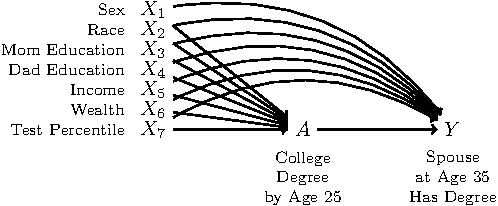
\includegraphics{models_for_causal_files/figure-pdf/unnamed-chunk-2-1.pdf}

By adjusting for the variables \(\vec{X}\), we block all non-causal
paths between the treatment \(A\) and the outcome \(Y\) in the DAG. If
this DAG is correct, then conditional exchangeability holds with this
adjustment set: \(\{Y^1,Y^0\}\indep A \mid\vec{X}\).

To estimate, we use data from the
\href{https://www.bls.gov/nls/nlsy97.htm}{National Longitudinal Survey
of Youth 1997}, a probability sample of U.S. resident children who were
ages 12--16 on Dec 31, 1996. The study followed these children and
interviewed them every year through 2011 and then every other year after
that.

We will analyze a simulated version of these data
(\href{../data/nlsy97_simulated.csv}{nlsy97\_simulated.csv}), which you
can access with this line of code.

\begin{Shaded}
\begin{Highlighting}[]
\NormalTok{all\_cases }\OtherTok{\textless{}{-}} \FunctionTok{read\_csv}\NormalTok{(}\StringTok{"https://soc114.github.io/data/nlsy97\_simulated.csv"}\NormalTok{)}
\end{Highlighting}
\end{Shaded}

\begin{tcolorbox}[enhanced jigsaw, leftrule=.75mm, breakable, opacityback=0, opacitybacktitle=0.6, colframe=quarto-callout-note-color-frame, toprule=.15mm, bottomrule=.15mm, rightrule=.15mm, colbacktitle=quarto-callout-note-color!10!white, arc=.35mm, colback=white, titlerule=0mm, left=2mm, toptitle=1mm, bottomtitle=1mm, title=\textcolor{quarto-callout-note-color}{\faInfo}\hspace{0.5em}{Expand to learn how to get the actual data}, coltitle=black]

To access the actual data, you would need to
\href{https://nlsinfo.org/investigator/pages/register}{register} for an
account, \href{https://nlsinfo.org/investigator/pages/login}{log in},
upload the \href{../code/nlsy97.NLSY97}{nlsy97.NLSY97} tagset that
identifies our variables, and then download. Unzip the folder and put
the contents in a directory on your computer. Then run our code file
\href{../code/prepare_nlsy97.R}{prepare\_nlsy97.R} in that folder. This
will produce a new file \texttt{d.RDS}, contains the data. You could
analyze that file. In the interest of transparency, we wrote the code
\href{../data/nlsy97_simulated.R}{nlsy97\_simulated.R} to convert these
real data to simulated data that we can share.

\end{tcolorbox}

The data contain several variables

\begin{itemize}
\tightlist
\item
  \texttt{id} is an individual identifier for each person
\item
  \texttt{a} is the treatment, containing the respondent's education
  coded \texttt{treated} if the respondent completed a four-year college
  degree and \texttt{untreated} if not.
\item
  \texttt{y} is the outcome: \texttt{TRUE} if has a spouse or
  residential partner at age 35 who holds a college degree, and
  \texttt{FALSE} if no spouse or partner or if the spouse or partner at
  age 35 does not have a degree.
\item
  There are several pre-treatment variables

  \begin{itemize}
  \tightlist
  \item
    \texttt{sex} is coded \texttt{Female} and \texttt{Male}
  \item
    \texttt{race} is race/ethnicity and is coded \texttt{Hispanic},
    \texttt{Non-Hispanic\ Black}, and \texttt{Non-Hispanic\ Non-Black}.
  \item
    \texttt{mom\_educ} is the respondent's mother's education as
    reported in 1997. It takes the value \texttt{No\ mom} if the child
    had no residential mother in 1997, and otherwise is coded with her
    education: \texttt{\textless{}\ HS}, \texttt{High\ school},
    \texttt{Some\ college}, or \texttt{College}.
  \item
    \texttt{dad\_educ} is the respondent's father's education as
    reported in 1997. It takes the value \texttt{No\ dad} if the child
    had no residential father in 1997, and otherwise is coded with his
    education: \texttt{\textless{}\ HS}, \texttt{High\ school},
    \texttt{Some\ college}, or \texttt{College}.
  \item
    \texttt{log\_parent\_income} is the log of gross household income in
    1997
  \item
    \texttt{log\_parent\_wealth} is the log of household net worth in
    1997
  \item
    \texttt{test\_percentile} is the respondent's percentile score on a
    test of math and verbal skills administered in 1999 (the Armed
    Services Vocational Aptitude Battery).
  \end{itemize}
\end{itemize}

When values are missing, we have replcaed them with predicted values. In
the simulated data, no row represents a real person because values have
been drawn randomly from a probability distribution designed to mimic
what exists in the real data. As discussed above, we did this in order
to share the file with you by a download on this website.

\subsection{Outcome modeling}\label{outcome-modeling}

Because the causal effect of \texttt{A} on \texttt{Y} is identified by
adjusting for the confounders, we can estimate by outcome modeling.
There are three general steps.

\begin{enumerate}
\def\labelenumi{\arabic{enumi})}
\tightlist
\item
  Model \(E(Y\mid A, \vec{X})\), the conditional mean of \(Y\) given the
  treatment and confounders
\item
  Predict potential outcomes

  \begin{itemize}
  \tightlist
  \item
    Predict \(Y^1\) for every unit
  \item
    Predict \(Y^0\) for every unit
  \end{itemize}
\item
  Aggregate to the average causal effect
\end{enumerate}

\subsubsection{With one confounder}\label{with-one-confounder}

We first illustrate the steps as though there were only one confounding
variable: test percentile. The first step is to create a data object
containing only the treated observations and a data object containing
only the untreated observations.

\begin{Shaded}
\begin{Highlighting}[]
\NormalTok{untreated\_cases }\OtherTok{\textless{}{-}}\NormalTok{ all\_cases }\SpecialCharTok{|\textgreater{}} \FunctionTok{filter}\NormalTok{(a }\SpecialCharTok{==} \StringTok{"untreated"}\NormalTok{)}
\NormalTok{treated\_cases }\OtherTok{\textless{}{-}}\NormalTok{ all\_cases }\SpecialCharTok{|\textgreater{}} \FunctionTok{filter}\NormalTok{(a }\SpecialCharTok{==} \StringTok{"treated"}\NormalTok{)}
\end{Highlighting}
\end{Shaded}

We use the untreated cases to estimate a model for \(Y^0\) as a function
of \(X\). If our data include sampling weights, then we weight this
model by the sampling weights.

\begin{Shaded}
\begin{Highlighting}[]
\NormalTok{model\_for\_y0 }\OtherTok{\textless{}{-}} \FunctionTok{lm}\NormalTok{(}
\NormalTok{  y }\SpecialCharTok{\textasciitilde{}}\NormalTok{ test\_percentile, }
  \AttributeTok{data =}\NormalTok{ untreated\_cases,}
  \AttributeTok{weights =}\NormalTok{ sampling\_weight}
\NormalTok{)}
\end{Highlighting}
\end{Shaded}

What happened above? The \texttt{lm()} function estimates a linear
model, which is stored in the \texttt{model} object. The first argument
is the model formula, which defines the function by which we model the
conditional mean of the outcome given the predictors. The second
argument is the data we use to learn the model.

In math, this model could be written as, \[
\text{E}(Y\mid A = 0, X) = \alpha_0 + \beta_0 X
\] where \(\alpha_0\) is an intercept and \(\beta_0\) is a slope. Here,
we are using the 0 subscripts to denote that these are estimates among
the untreated.

We can likewise use the treated cases to estimate a model for \(Y^1\) as
a function of \(X\).

\begin{Shaded}
\begin{Highlighting}[]
\NormalTok{model\_for\_y1 }\OtherTok{\textless{}{-}} \FunctionTok{lm}\NormalTok{(}
\NormalTok{  y }\SpecialCharTok{\textasciitilde{}}\NormalTok{ test\_percentile, }
  \AttributeTok{data =}\NormalTok{ treated\_cases,}
  \AttributeTok{weights =}\NormalTok{ sampling\_weight}
\NormalTok{)}
\end{Highlighting}
\end{Shaded}

which could be written in math as follows.

\[
\text{E}(Y\mid A = 1, X) = \alpha_1 + \beta_1 X
\]

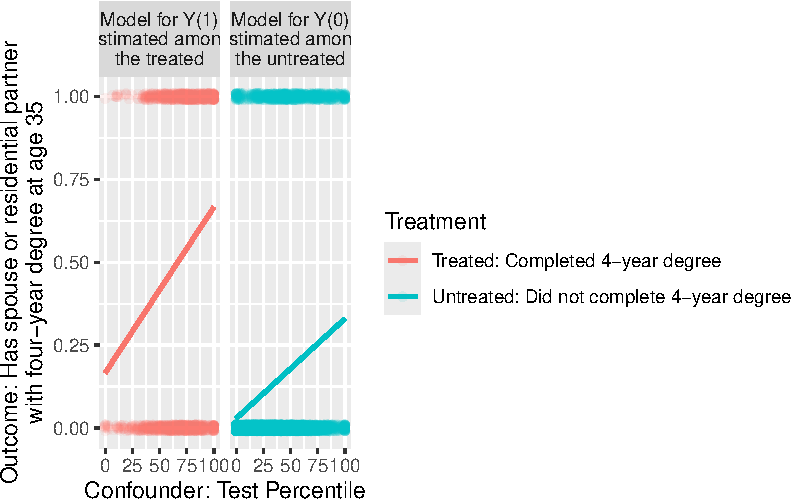
\includegraphics{models_for_causal_files/figure-pdf/unnamed-chunk-8-1.pdf}

We can now use our models to predict for our target population. For the
average treatment effect, the target population is all cases. For every
case, we can predict probabilities under treatment and under control.

\[
\begin{aligned}
\hat{Y}_1 &= \hat{\text{E}}(Y\mid A = 1, X) = \hat\alpha_1 + \hat\beta_1 X \\
\hat{Y}_0 &= \hat{\text{E}}(Y\mid A = 0, X) = \hat\alpha_0 + \hat\beta_0 X \\
\end{aligned}
\]

In code, we make those predictions with the \texttt{predict()} function,
storing them in new variables \texttt{yhat1} and \texttt{yhat0}.

\begin{Shaded}
\begin{Highlighting}[]
\NormalTok{predicted\_potential\_outcomes }\OtherTok{\textless{}{-}}\NormalTok{ all\_cases }\SpecialCharTok{|\textgreater{}}
  \FunctionTok{mutate}\NormalTok{(}
    \AttributeTok{yhat1 =} \FunctionTok{predict}\NormalTok{(model\_for\_y1, }\AttributeTok{newdata =}\NormalTok{ all\_cases),}
    \AttributeTok{yhat0 =} \FunctionTok{predict}\NormalTok{(model\_for\_y0, }\AttributeTok{newdata =}\NormalTok{ all\_cases),}
    \AttributeTok{effect =}\NormalTok{ yhat1 }\SpecialCharTok{{-}}\NormalTok{ yhat0}
\NormalTok{  )}
\end{Highlighting}
\end{Shaded}

\begin{verbatim}
# A tibble: 7,688 x 6
     id sampling_weight a         yhat1  yhat0 effect
  <dbl>           <dbl> <chr>     <dbl>  <dbl>  <dbl>
1     1           0.989 untreated 0.403 0.171   0.232
2     2           0.999 treated   0.645 0.317   0.328
3     3           0.967 untreated 0.283 0.0990  0.184
# i 7,685 more rows
\end{verbatim}

Visually, the target population is all the gray points: everyone
regardless of treatment. For each point, we predict the outcome
probability under treatment and under no treatment.

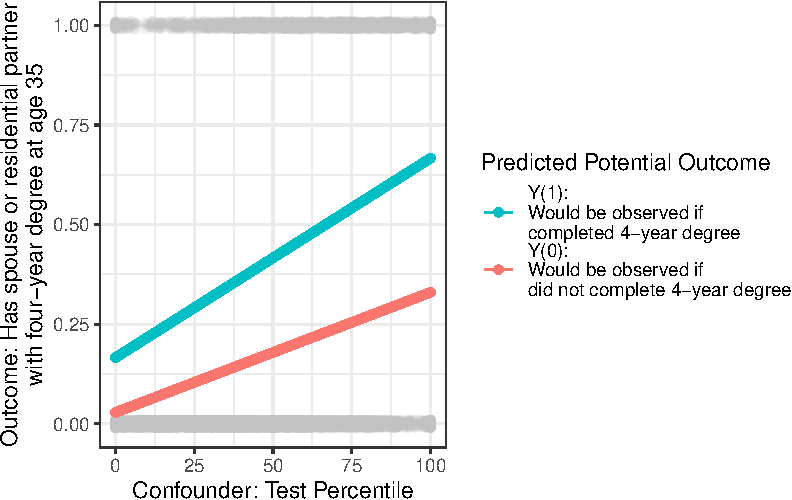
\includegraphics{models_for_causal_files/figure-pdf/unnamed-chunk-11-1.pdf}

The average treatment effect (ATE) is the weighted average of the
case-specific effect estimates, weighted by sampling weights.

\begin{Shaded}
\begin{Highlighting}[]
\NormalTok{predicted\_potential\_outcomes }\SpecialCharTok{|\textgreater{}}
  \FunctionTok{summarize}\NormalTok{(}\AttributeTok{ate =} \FunctionTok{weighted.mean}\NormalTok{(effect, }\AttributeTok{w =}\NormalTok{ sampling\_weight))}
\end{Highlighting}
\end{Shaded}

\begin{verbatim}
# A tibble: 1 x 1
    ate
  <dbl>
1 0.224
\end{verbatim}

We could also estimate among any subgroup, for example the average
treatment effect among the treated and among the untreated.

\begin{Shaded}
\begin{Highlighting}[]
\NormalTok{predicted\_potential\_outcomes }\SpecialCharTok{|\textgreater{}}
  \FunctionTok{group\_by}\NormalTok{(a) }\SpecialCharTok{|\textgreater{}}
  \FunctionTok{summarize}\NormalTok{(}\AttributeTok{conditional\_average\_effect =} \FunctionTok{weighted.mean}\NormalTok{(effect, }\AttributeTok{w =}\NormalTok{ sampling\_weight))}
\end{Highlighting}
\end{Shaded}

\begin{verbatim}
# A tibble: 2 x 2
  a         conditional_average_effect
  <chr>                          <dbl>
1 treated                        0.278
2 untreated                      0.211
\end{verbatim}

\subsubsection{With many confounders}\label{with-many-confounders}

Outcome modeling generalizes easily from one confounder to many
confounders. The only change is to include more confounders in the
outcome model formulas.

\begin{Shaded}
\begin{Highlighting}[]
\NormalTok{model\_for\_y0 }\OtherTok{\textless{}{-}} \FunctionTok{lm}\NormalTok{(}
\NormalTok{  y }\SpecialCharTok{\textasciitilde{}}\NormalTok{ sex }\SpecialCharTok{+}\NormalTok{ race }\SpecialCharTok{+}\NormalTok{ mom\_educ }\SpecialCharTok{+}\NormalTok{ dad\_educ }\SpecialCharTok{+}\NormalTok{ log\_parent\_income }\SpecialCharTok{+}
\NormalTok{    log\_parent\_wealth }\SpecialCharTok{+}\NormalTok{ test\_percentile, }
  \AttributeTok{data =}\NormalTok{ untreated\_cases,}
  \AttributeTok{weights =}\NormalTok{ sampling\_weight}
\NormalTok{)}
\NormalTok{model\_for\_y1 }\OtherTok{\textless{}{-}} \FunctionTok{lm}\NormalTok{(}
\NormalTok{  y }\SpecialCharTok{\textasciitilde{}}\NormalTok{ sex }\SpecialCharTok{+}\NormalTok{ race }\SpecialCharTok{+}\NormalTok{ mom\_educ }\SpecialCharTok{+}\NormalTok{ dad\_educ }\SpecialCharTok{+}\NormalTok{ log\_parent\_income }\SpecialCharTok{+}
\NormalTok{    log\_parent\_wealth }\SpecialCharTok{+}\NormalTok{ test\_percentile, }
  \AttributeTok{data =}\NormalTok{ treated\_cases,}
  \AttributeTok{weights =}\NormalTok{ sampling\_weight}
\NormalTok{)}
\end{Highlighting}
\end{Shaded}

Otherwise, outcome modeling with many confounders follows the same
process. If our goal is to estimate the average treatment effect in
\texttt{all\_cases},

\begin{Shaded}
\begin{Highlighting}[]
\NormalTok{predicted\_potential\_outcomes }\OtherTok{\textless{}{-}}\NormalTok{ all\_cases }\SpecialCharTok{|\textgreater{}}
  \FunctionTok{mutate}\NormalTok{(}
    \AttributeTok{yhat1 =} \FunctionTok{predict}\NormalTok{(model\_for\_y1, }\AttributeTok{newdata =}\NormalTok{ all\_cases),}
    \AttributeTok{yhat0 =} \FunctionTok{predict}\NormalTok{(model\_for\_y0, }\AttributeTok{newdata =}\NormalTok{ all\_cases),}
    \AttributeTok{effect =}\NormalTok{ yhat1 }\SpecialCharTok{{-}}\NormalTok{ yhat0}
\NormalTok{  ) }\SpecialCharTok{|\textgreater{}}
  \FunctionTok{select}\NormalTok{(id, sampling\_weight, a, yhat1, yhat0, effect) }\SpecialCharTok{|\textgreater{}}
  \FunctionTok{print}\NormalTok{(}\AttributeTok{n =} \DecValTok{3}\NormalTok{)}
\end{Highlighting}
\end{Shaded}

\begin{verbatim}
# A tibble: 7,688 x 6
     id sampling_weight a         yhat1   yhat0 effect
  <dbl>           <dbl> <chr>     <dbl>   <dbl>  <dbl>
1     1           0.989 untreated 0.255  0.0889  0.166
2     2           0.999 treated   0.727  0.441   0.285
3     3           0.967 untreated 0.149 -0.0139  0.163
# i 7,685 more rows
\end{verbatim}

The average treatment effect (ATE) is the weighted average of the
case-specific effect estimates, weighted by sampling weights.

\begin{Shaded}
\begin{Highlighting}[]
\NormalTok{predicted\_potential\_outcomes }\SpecialCharTok{|\textgreater{}}
  \FunctionTok{summarize}\NormalTok{(}\AttributeTok{ate =} \FunctionTok{weighted.mean}\NormalTok{(effect, }\AttributeTok{w =}\NormalTok{ sampling\_weight))}
\end{Highlighting}
\end{Shaded}

\begin{verbatim}
# A tibble: 1 x 1
    ate
  <dbl>
1 0.199
\end{verbatim}

We could also estimate among any subgroup, for example the average
treatment effect among the treated and among the untreated.

\begin{Shaded}
\begin{Highlighting}[]
\NormalTok{predicted\_potential\_outcomes }\SpecialCharTok{|\textgreater{}}
  \FunctionTok{group\_by}\NormalTok{(a) }\SpecialCharTok{|\textgreater{}}
  \FunctionTok{summarize}\NormalTok{(}\AttributeTok{conditional\_average\_effect =} \FunctionTok{weighted.mean}\NormalTok{(effect, }\AttributeTok{w =}\NormalTok{ sampling\_weight))}
\end{Highlighting}
\end{Shaded}

\begin{verbatim}
# A tibble: 2 x 2
  a         conditional_average_effect
  <chr>                          <dbl>
1 treated                        0.253
2 untreated                      0.187
\end{verbatim}

\subsubsection{Generalizing to logistic
regression}\label{generalizing-to-logistic-regression}

In the illustration above, we might be concerned that our outcome is
binary (taking values 0 or 1) and yet the predictions are sometimes
below 0 or above 1.

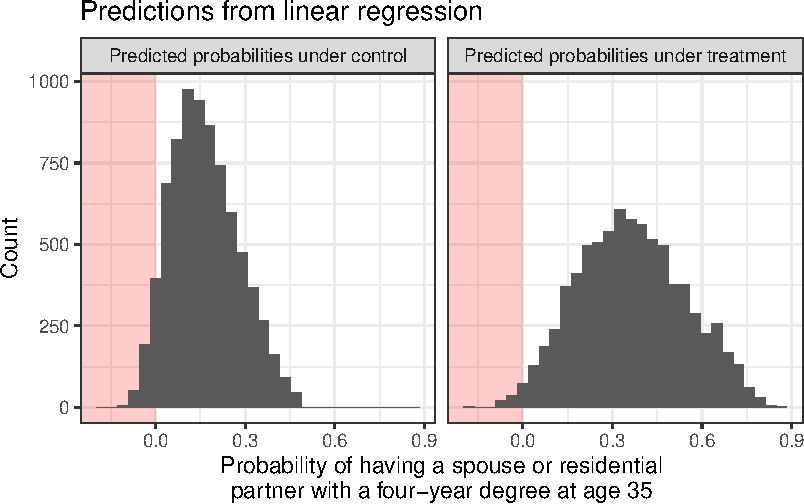
\includegraphics{models_for_causal_files/figure-pdf/unnamed-chunk-18-1.pdf}

Both models are predicting that some people have \textbf{negative}
probabilities of having a college-degree-holding spouse or partner! We
might want to solve this by estimating logistic regression models. We do
this with the \texttt{glm()} function with the argument
\texttt{family\ =\ binomial}.

\begin{quote}
If logistic regression is new to you, see the bottom of
\href{what_is_a_model.qmd}{What is a model?}.
\end{quote}

\begin{Shaded}
\begin{Highlighting}[]
\NormalTok{logistic\_model\_for\_y0 }\OtherTok{\textless{}{-}} \FunctionTok{glm}\NormalTok{(}
\NormalTok{  y }\SpecialCharTok{\textasciitilde{}}\NormalTok{ sex }\SpecialCharTok{+}\NormalTok{ race }\SpecialCharTok{+}\NormalTok{ mom\_educ }\SpecialCharTok{+}\NormalTok{ dad\_educ }\SpecialCharTok{+}\NormalTok{ log\_parent\_income }\SpecialCharTok{+}
\NormalTok{    log\_parent\_wealth }\SpecialCharTok{+}\NormalTok{ test\_percentile, }
  \AttributeTok{family =}\NormalTok{ binomial,}
  \AttributeTok{data =}\NormalTok{ untreated\_cases,}
  \AttributeTok{weights =}\NormalTok{ sampling\_weight}
\NormalTok{)}
\end{Highlighting}
\end{Shaded}

\begin{verbatim}
Warning in eval(family$initialize): non-integer #successes in a binomial glm!
\end{verbatim}

\begin{Shaded}
\begin{Highlighting}[]
\NormalTok{logistic\_model\_for\_y1 }\OtherTok{\textless{}{-}} \FunctionTok{glm}\NormalTok{(}
\NormalTok{  y }\SpecialCharTok{\textasciitilde{}}\NormalTok{ sex }\SpecialCharTok{+}\NormalTok{ race }\SpecialCharTok{+}\NormalTok{ mom\_educ }\SpecialCharTok{+}\NormalTok{ dad\_educ }\SpecialCharTok{+}\NormalTok{ log\_parent\_income }\SpecialCharTok{+}
\NormalTok{    log\_parent\_wealth }\SpecialCharTok{+}\NormalTok{ test\_percentile, }
  \AttributeTok{family =}\NormalTok{ binomial,}
  \AttributeTok{data =}\NormalTok{ treated\_cases,}
  \AttributeTok{weights =}\NormalTok{ sampling\_weight}
\NormalTok{)}
\end{Highlighting}
\end{Shaded}

\begin{verbatim}
Warning in eval(family$initialize): non-integer #successes in a binomial glm!
\end{verbatim}

These models return a warning that there is a non-integer number of
successes. This is normal and not a concern when estimating logistic
regression models with weights.

Just as with linear regression, we can use our logistic regression to
predict potential outcome values. When making predictions, it is
important to use the \texttt{type\ =\ "response"} argument to predict
the probability of \(Y = 1\) instead of the log odds of \(Y = 1\).

\begin{Shaded}
\begin{Highlighting}[]
\NormalTok{logistic\_predicted\_potential\_outcomes }\OtherTok{\textless{}{-}}\NormalTok{ all\_cases }\SpecialCharTok{|\textgreater{}}
  \FunctionTok{mutate}\NormalTok{(}
    \AttributeTok{yhat1 =} \FunctionTok{predict}\NormalTok{(}
\NormalTok{      logistic\_model\_for\_y1, }
      \AttributeTok{newdata =}\NormalTok{ all\_cases, }
      \AttributeTok{type =} \StringTok{"response"}
\NormalTok{    ),}
    \AttributeTok{yhat0 =} \FunctionTok{predict}\NormalTok{(}
\NormalTok{      logistic\_model\_for\_y0, }
      \AttributeTok{newdata =}\NormalTok{ all\_cases, }
      \AttributeTok{type =} \StringTok{"response"}
\NormalTok{    ),}
    \AttributeTok{effect =}\NormalTok{ yhat1 }\SpecialCharTok{{-}}\NormalTok{ yhat0}
\NormalTok{  )}
\end{Highlighting}
\end{Shaded}

\begin{verbatim}
# A tibble: 7,688 x 6
     id sampling_weight a         yhat1  yhat0 effect
  <dbl>           <dbl> <chr>     <dbl>  <dbl>  <dbl>
1     1           0.989 untreated 0.254 0.0861  0.168
2     2           0.999 treated   0.726 0.562   0.164
3     3           0.967 untreated 0.177 0.0261  0.151
# i 7,685 more rows
\end{verbatim}

In math, we can see why the \texttt{type\ =\ "response"} is needed. By
default, using \texttt{predict()} after logistic regression will predict
the log odds of the outcome. For example for the outcome under
treatment:

\[
\log\left(\frac{\hat{\text{P}}(Y = 1\mid A = 1, X)}{1 - \hat{\text{P}}(Y = 1\mid A = 1, X)}\right) = \hat\alpha_1 + \hat\beta_1 X
\]

But we really estimated the model to estimate
\(\hat{P}(Y = 1\mid A = 1, X)\), not a complicated function of that
quantity. By typing \texttt{type\ =\ "response"}, you tell R to invert
the logit function and return predicted probabilities.

\[
\hat{\text{P}}(Y = 1\mid A = 1, X) = \frac{e^{\hat\alpha_1 + \hat\beta_1 X}}{1 + e^{\hat\alpha_1 + \hat\beta_1 X}}
\]

By using \texttt{type\ =\ "response"}, you can think about the
probabilities on the left side of the equation and not the math on the
right side of the equation. We can visualize that with logistic
regression, all predicted probabilities fall within the {[}0,1{]} range.

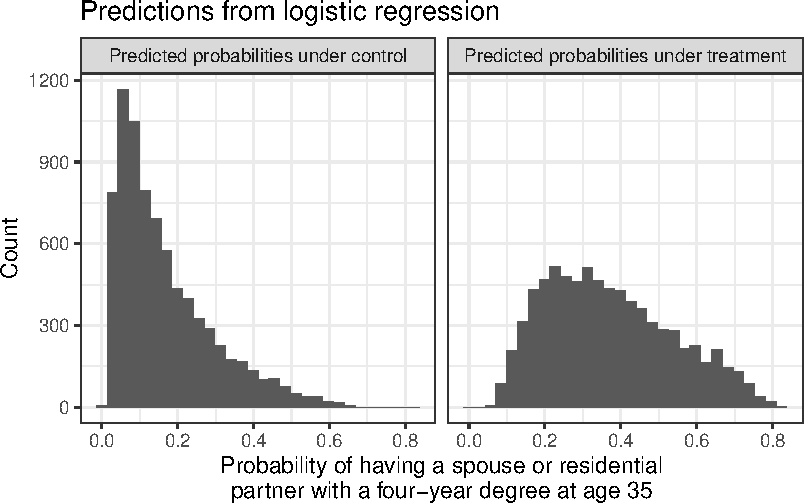
\includegraphics{models_for_causal_files/figure-pdf/unnamed-chunk-22-1.pdf}

Exactly as with linear regression, we can aggregate the predicted
potential outcomes to estimate the average treatment effect over all
cases (ATT),

\begin{Shaded}
\begin{Highlighting}[]
\NormalTok{logistic\_ate\_estimate }\OtherTok{\textless{}{-}}\NormalTok{ logistic\_predicted\_potential\_outcomes }\SpecialCharTok{|\textgreater{}}
  \FunctionTok{summarize}\NormalTok{(}\AttributeTok{ate =} \FunctionTok{weighted.mean}\NormalTok{(effect, }\AttributeTok{w =}\NormalTok{ sampling\_weight)) }\SpecialCharTok{|\textgreater{}}
  \FunctionTok{print}\NormalTok{()}
\end{Highlighting}
\end{Shaded}

\begin{verbatim}
# A tibble: 1 x 1
    ate
  <dbl>
1 0.204
\end{verbatim}

or among those who were factually treated or untreated,

\begin{Shaded}
\begin{Highlighting}[]
\NormalTok{logistic\_predicted\_potential\_outcomes }\SpecialCharTok{|\textgreater{}}
  \FunctionTok{group\_by}\NormalTok{(a) }\SpecialCharTok{|\textgreater{}}
  \FunctionTok{summarize}\NormalTok{(}\AttributeTok{conditional\_average\_effect =} \FunctionTok{weighted.mean}\NormalTok{(effect, }\AttributeTok{w =}\NormalTok{ sampling\_weight))}
\end{Highlighting}
\end{Shaded}

\begin{verbatim}
# A tibble: 2 x 2
  a         conditional_average_effect
  <chr>                          <dbl>
1 treated                        0.240
2 untreated                      0.195
\end{verbatim}

or among any subpopulation by grouping by any confounding variables.

We estimate that completing college increases the probability of having
a college-educated by 0.204. This causal conclusion relies both on our
causal assumptions (the DAG) and our statistical assumptions (the chosen
model).

\subsection{Treatment modeling}\label{treatment-modeling}

Instead of modeling the outcome, another way of using models for causal
inference is to model the probability of treatment assignment. This
approach is more analogous to sampling from a population.

In a probability sample, we observe the outcome \(Y_i\) for any sampled
unit \((S_i=1)\) which is seen with some probability of sampling,
\(P(S=1\mid\vec{X} = \vec{x}_i)\) that may differ across subgroups with
different values of some variables \(\vec{X}\). As discussed in
population sampling, the sampling weight is the inverse of these
probabilities. A person who is sampled with a 20\% probability
represents 1 / .2 = 5 people in the population (the other 4 being
unsampled).

In a conditionally randomized experiment, we observe the outcome under
treatment \(Y_i^1\) for any treated unit \(A_i=1\), which might be
assigned with some probability \(P(A_i=1\mid\vec{X} = \vec{x}_i)\) that
differs across subgroups defined by an adjustment set \(\vec{X}\). In a
conditionally randomized experiment, these probabilities are known and
the overall expected outcome under treatment \(\text{E}(Y^1)\) can be
estimated by the average of the observed outcomes under treatment,
weighted by the inverse probability of being treated. A treated unit who
had a 20\% probability of being treated represents 1 / .2 = 5 people
(the other 4 being untreated).

In an observational study, we don't know the probability of being
treated given the variables in our sufficient adjustment set. We need to
model that probability. There are three general steps.

\begin{enumerate}
\def\labelenumi{\arabic{enumi})}
\tightlist
\item
  Model treatment probabilities given an adjustment set
\item
  Construct a weight for each unit
\item
  Estimate by weighted means within each treatment group
\end{enumerate}

\subsubsection{1) Model treatment
probabilities}\label{model-treatment-probabilities}

One way to model the probability of treatment is with logistic
regression. If logistic regression is new to you, see the bottom of
\href{what_is_a_model.qmd}{What is a model?}.

\[
\log\left(\frac{P(A = 1 \mid\vec{X})}{1-P(A = 1\mid\vec{X})}\right) = \alpha + \vec{X}'\vec\beta
\]

\begin{Shaded}
\begin{Highlighting}[]
\NormalTok{treatment\_model }\OtherTok{\textless{}{-}} \FunctionTok{glm}\NormalTok{(}
  \FunctionTok{I}\NormalTok{(a }\SpecialCharTok{==} \StringTok{"treated"}\NormalTok{) }\SpecialCharTok{\textasciitilde{}}\NormalTok{ sex }\SpecialCharTok{+}\NormalTok{ race }\SpecialCharTok{+}\NormalTok{ mom\_educ }\SpecialCharTok{+}\NormalTok{ dad\_educ }\SpecialCharTok{+}\NormalTok{ log\_parent\_income }\SpecialCharTok{+}
\NormalTok{    log\_parent\_wealth }\SpecialCharTok{+}\NormalTok{ test\_percentile,}
  \AttributeTok{family =}\NormalTok{ binomial,}
  \AttributeTok{data =}\NormalTok{ all\_cases}
\NormalTok{)}
\end{Highlighting}
\end{Shaded}

For every unit, we can then predict the probability of being treated
given the adjustment set.

\begin{Shaded}
\begin{Highlighting}[]
\NormalTok{predicted\_treatment\_probabilities }\OtherTok{\textless{}{-}}\NormalTok{ all\_cases }\SpecialCharTok{|\textgreater{}}
  \FunctionTok{mutate}\NormalTok{(}\AttributeTok{p\_treated =} \FunctionTok{predict}\NormalTok{(treatment\_model, }\AttributeTok{type =} \StringTok{"response"}\NormalTok{)) }\SpecialCharTok{|\textgreater{}}
  \FunctionTok{select}\NormalTok{(id, a, y, p\_treated)}
\end{Highlighting}
\end{Shaded}

\begin{verbatim}
# A tibble: 7,688 x 4
     id a         y     p_treated
  <dbl> <chr>     <lgl>     <dbl>
1     1 untreated FALSE    0.0720
2     2 treated   TRUE     0.777 
3     3 untreated FALSE    0.0318
# i 7,685 more rows
\end{verbatim}

The \texttt{type\ =\ "response"} argument is essential, because this
tells R to predict the probability of treatment instead of the log odds
of treatment.

\subsubsection{2) Construct weights}\label{construct-weights}

For each unit, we can construct a weight that is the inverse probability
of that unit's treatment assignment. Recall that if a unit is treated
and had a 0.2 probability of treatment, then we could think of this unit
as representing 1 / 0.2 = 5 units: itself and 4 others like it who were
not treated. The weight on each unit is the inverse probability of the
treatment value that happened for that unit.

\[
w_i = \begin{cases}
\frac{1}{\text{P}(A = 1\mid \vec{X} = \vec{x}_i)} &\text{if treated} \\
\frac{1}{1 - \text{P}(A = 1\mid \vec{X} = \vec{x}_i)} &\text{if untreated}
\end{cases}
\]

In code, we can use \texttt{case\_when()} to assign this weight as
\texttt{1\ /\ p\_treated} for treated units and
\texttt{1\ /\ (1\ -\ p\_treated)} for untreated units.

\begin{Shaded}
\begin{Highlighting}[]
\NormalTok{inverse\_probability\_weights }\OtherTok{\textless{}{-}}\NormalTok{ predicted\_treatment\_probabilities }\SpecialCharTok{|\textgreater{}}
  \FunctionTok{mutate}\NormalTok{(}
    \AttributeTok{weight =} \FunctionTok{case\_when}\NormalTok{(}
\NormalTok{      a }\SpecialCharTok{==} \StringTok{"treated"} \SpecialCharTok{\textasciitilde{}} \DecValTok{1} \SpecialCharTok{/}\NormalTok{ p\_treated,}
\NormalTok{      a }\SpecialCharTok{==} \StringTok{"untreated"} \SpecialCharTok{\textasciitilde{}} \DecValTok{1} \SpecialCharTok{/}\NormalTok{ (}\DecValTok{1} \SpecialCharTok{{-}}\NormalTok{ p\_treated)}
\NormalTok{    )}
\NormalTok{  )}
\end{Highlighting}
\end{Shaded}

\begin{verbatim}
# A tibble: 7,688 x 5
     id a         y     p_treated weight
  <dbl> <chr>     <lgl>     <dbl>  <dbl>
1     1 untreated FALSE    0.0720   1.08
2     2 treated   TRUE     0.777    1.29
3     3 untreated FALSE    0.0318   1.03
# i 7,685 more rows
\end{verbatim}

\subsubsection{3) Estimate by weighted
means}\label{estimate-by-weighted-means}

Finally, we use the weights to take the treated units and draw inference
about what would happen to all units if they were hypothetically
treated, and to use the untreated units and draw inference about what
would happen to all units if they were hypothetically untreated.

\begin{Shaded}
\begin{Highlighting}[]
\NormalTok{inverse\_probability\_weights }\SpecialCharTok{|\textgreater{}}
  \CommentTok{\# Within each treatment group}
  \FunctionTok{group\_by}\NormalTok{(a) }\SpecialCharTok{|\textgreater{}}
  \CommentTok{\# Take the mean weighted by inverse probability of treatment weights}
  \FunctionTok{summarize}\NormalTok{(}\AttributeTok{estimate =} \FunctionTok{weighted.mean}\NormalTok{(y, }\AttributeTok{w =}\NormalTok{ weight)) }\SpecialCharTok{|\textgreater{}}
  \CommentTok{\# Pivot wider and difference to estimate the effect}
  \FunctionTok{pivot\_wider}\NormalTok{(}\AttributeTok{names\_from =}\NormalTok{ a, }\AttributeTok{values\_from =}\NormalTok{ estimate, }\AttributeTok{names\_prefix =} \StringTok{"if\_"}\NormalTok{) }\SpecialCharTok{|\textgreater{}}
  \FunctionTok{mutate}\NormalTok{(}\AttributeTok{effect =}\NormalTok{ if\_treated }\SpecialCharTok{{-}}\NormalTok{ if\_untreated)}
\end{Highlighting}
\end{Shaded}

\begin{verbatim}
# A tibble: 1 x 3
  if_treated if_untreated effect
       <dbl>        <dbl>  <dbl>
1      0.382        0.166  0.217
\end{verbatim}

\subsection{Concluding thoughts}\label{concluding-thoughts}

Outcome modeling is a powerful strategy because it bridges nonparametric
causal identification to longstanding strategies where outcomes are
modeled by parametric regression.

Inverse probability of treatment weighting is a powerful strategy
because it bridges nonparametric causal identification to longstanding
strategies from survey sampling where units from a population are
sampled with known probabilities of inclusion. The analogy is that
outcomes under treatment are sampled with estimated inclusion
probabilities (the probability of treatment). Just as in a population
sample we would need to think carefully about the probability of
sampling, treatment modeling encourages us to model the probability of
receiving the observed treatment.




\end{document}
